% !TeX root = ../../../main.tex
\begin{figure}[thb]\captionsetup{justification=raggedright,singlelinecheck=false}
\ChThreeFloatContents
  {ch03:fig:data_overview}
  {\caption{Overview of Schizophrenia Patient Trajectory in Allegheny County. (a) We look at the timing of the first composite outcome \(\in \{\text{\textcolor{orange}{Involuntary Hospitalization}, }\allowbreak\text{\textcolor{red}{Jail Stay}, }\allowbreak\text{\textbf{Death}}\}\). (b) Non-adherence at each month is calculated by looking at the daily equivalence of prescribed refills available for each month.}}
  {%
    \subfigure[Patient Trajectory]{\label{ch03:fig:patient_trajectory}%
      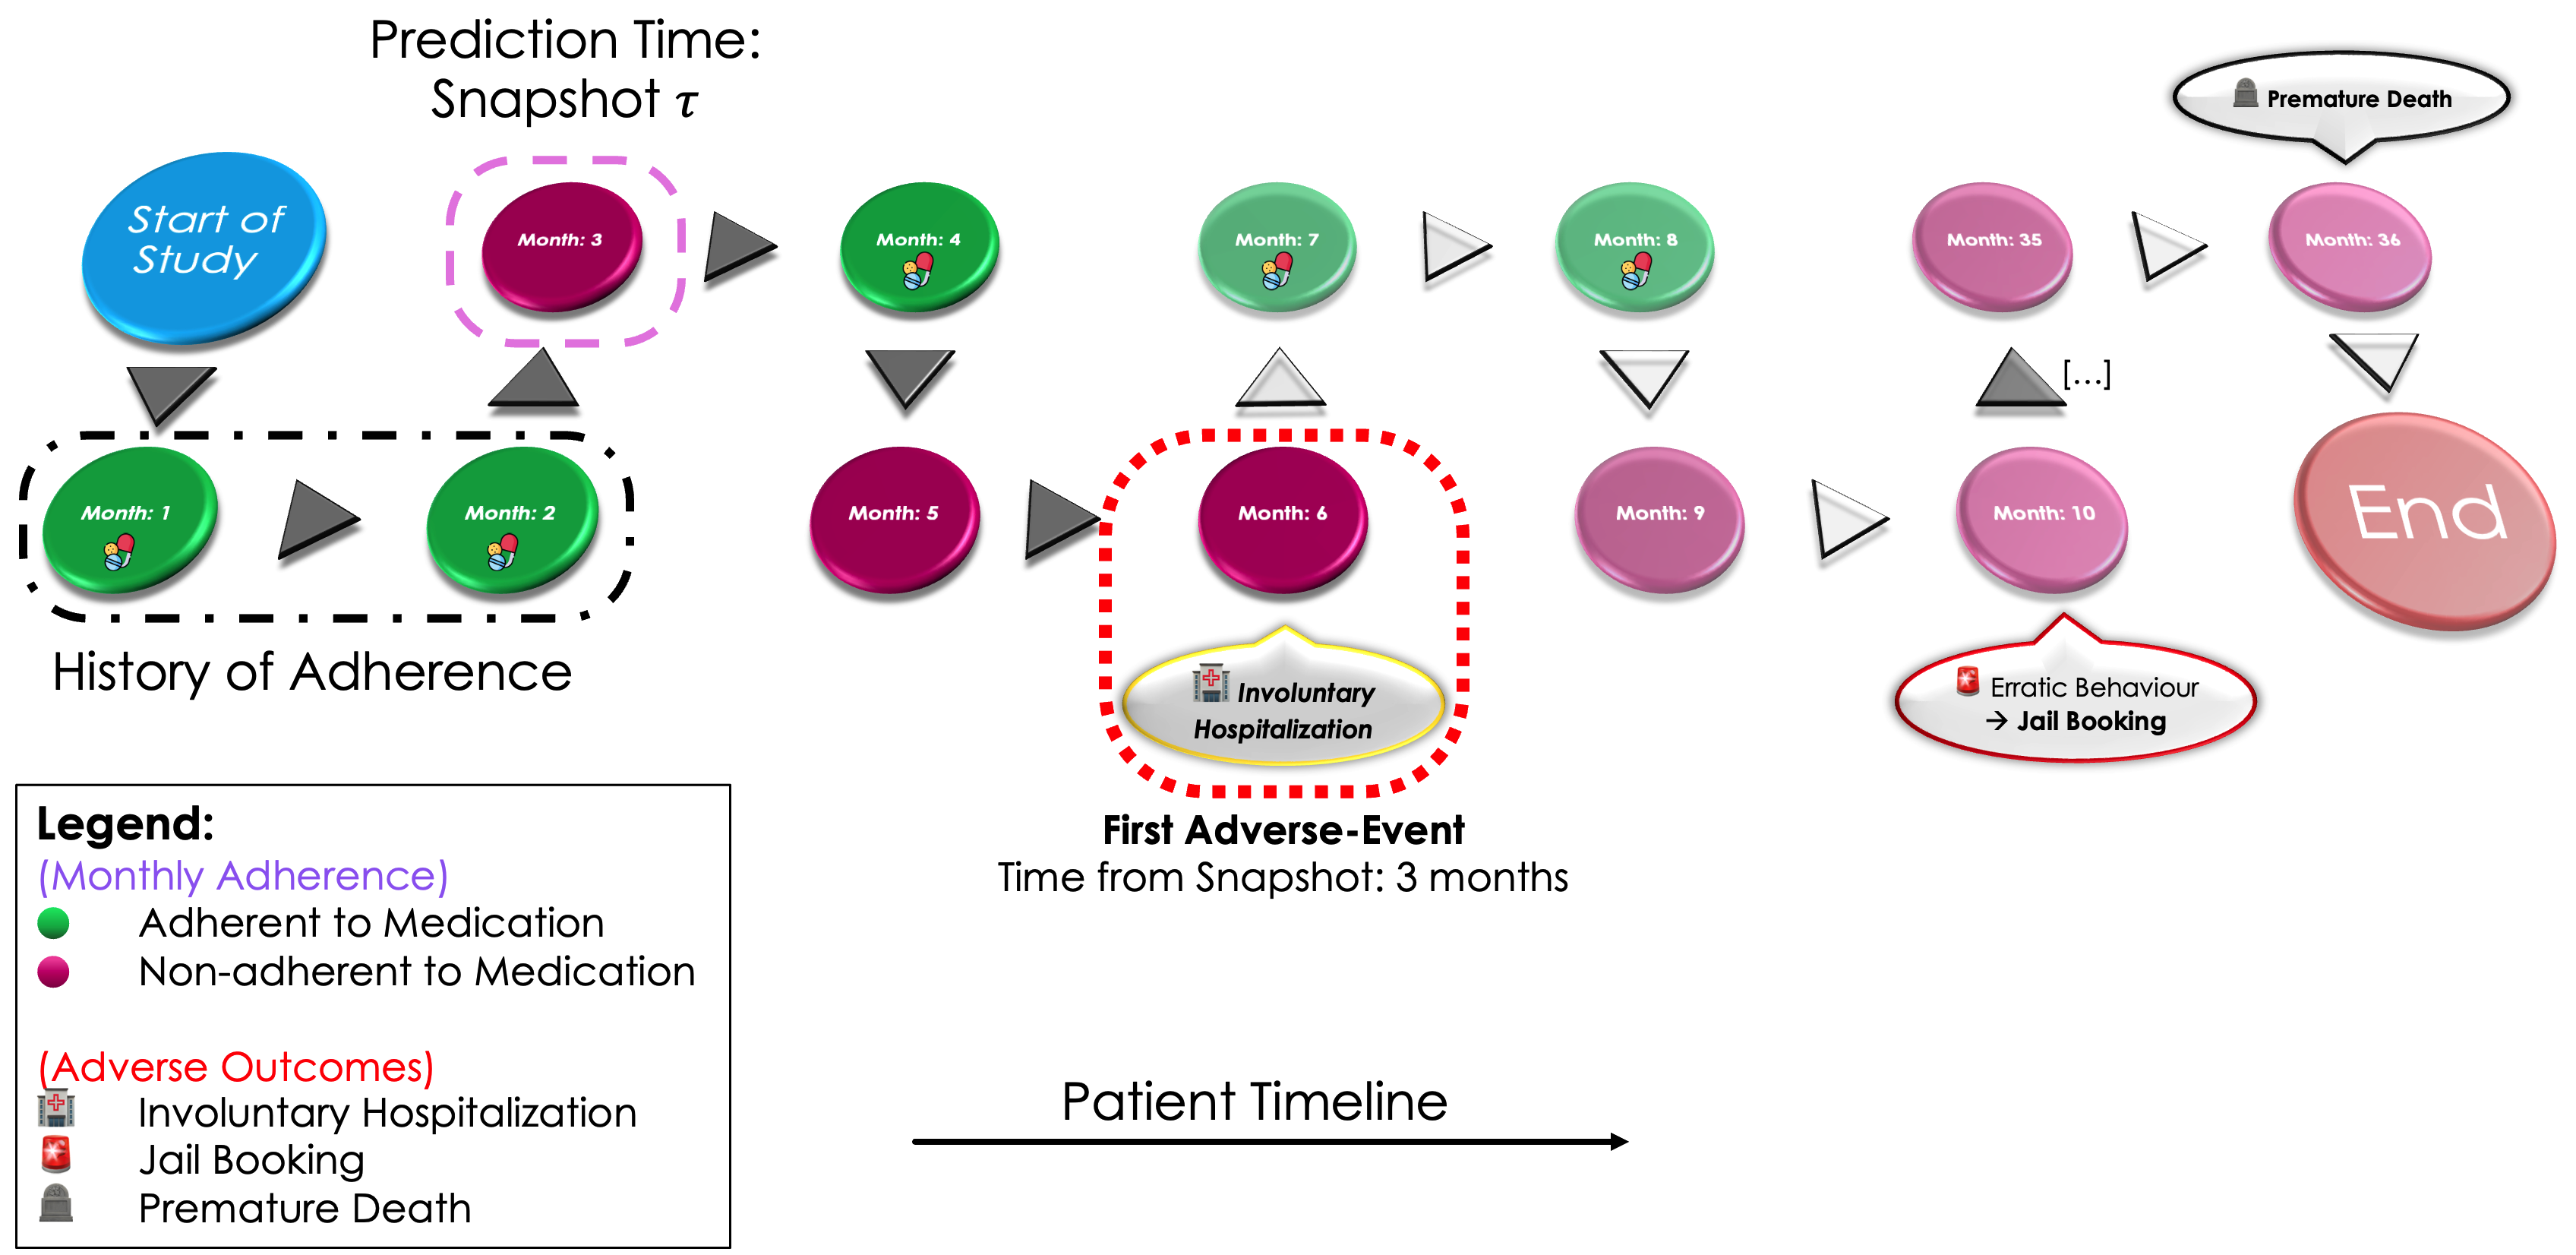
\includegraphics[width=.57\linewidth]{Appendices/appendix-ch03/images/Overview/Causal_Survival_Analysis-Patient_Trajectory.png}}%
    \hfill
    \subfigure[Gender]{\label{ch03:fig:adherence_indicator}%
      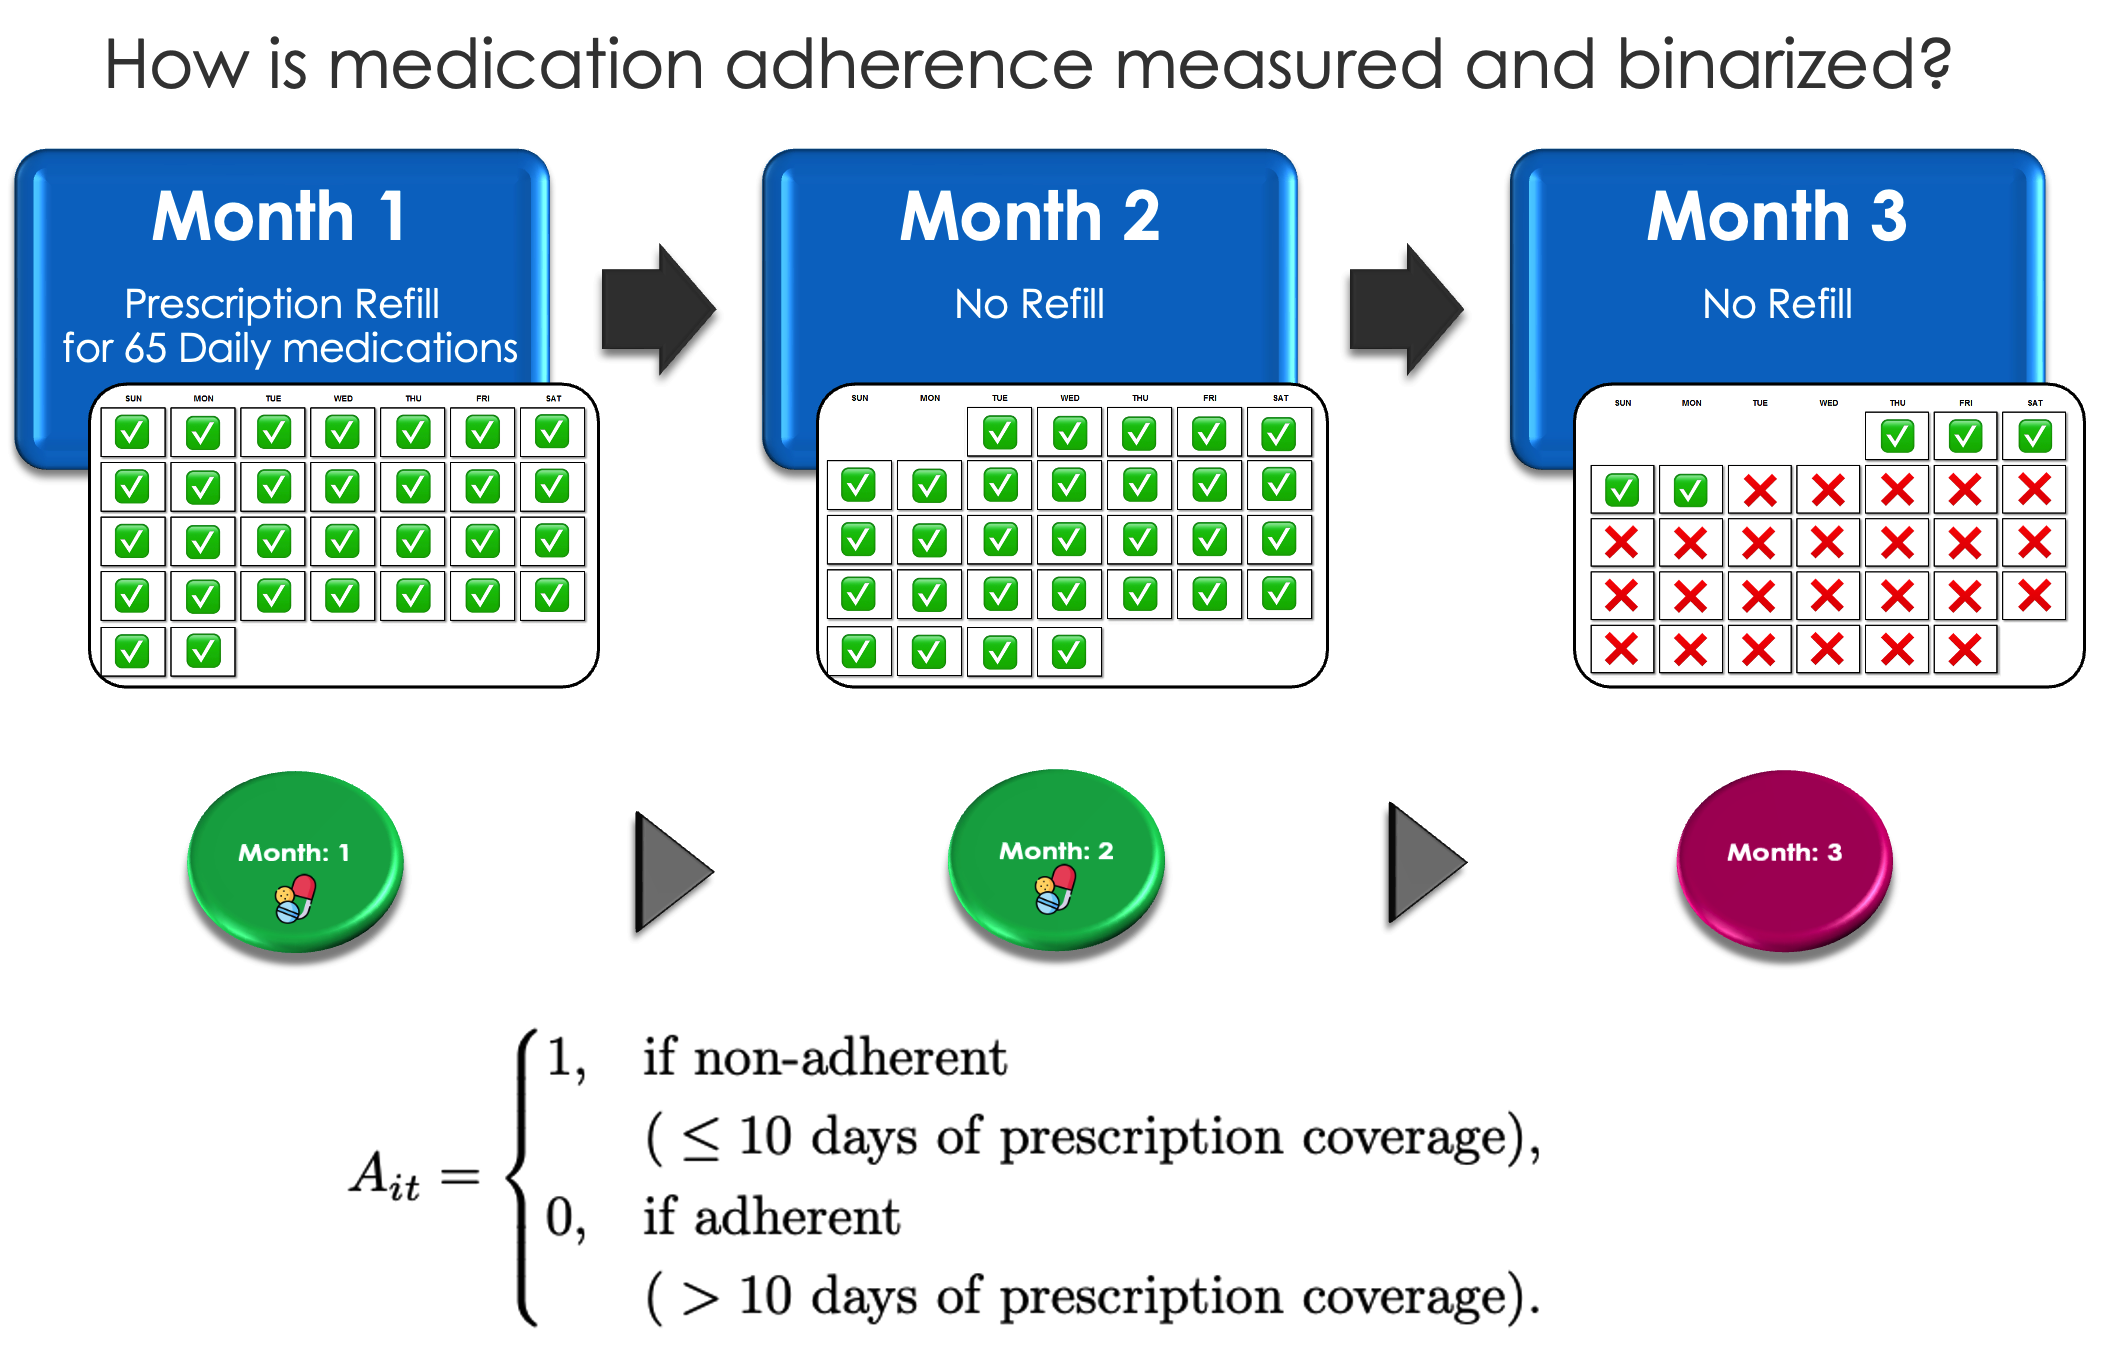
\includegraphics[width=.37\linewidth]{Appendices/appendix-ch03/images/Overview/Causal_Survival_Analysis-Adherence_Level.png}}%
    }
\end{figure}